\documentclass{article}
\usepackage{graphics}
\usepackage{amsmath,amssymb, mathtools}
\usepackage{amsfonts}
\usepackage{array}
\usepackage{multirow}
\usepackage{geometry}
\usepackage{hyperref}
\usepackage[utf8]{inputenc}
\usepackage[T2A]{fontenc}
%\usepackage[T2A, T1]{fontenc}


\begin{document}

\subsection*{Green-thing}

\[ a_nu^{n}(x)+\ldots +a_1u'(x)+a_0u(x) = f(x) \]

Găsim sol ec omogene (Neculasenpai style, doar ca acolo notam cu \(\lambda\), nu $r$):

radacinile polinomului caracteristic:
\[ a_n r^{n}+\ldots +a_1 + r a_1+a_0 = 0 \]

daca avem radacinile \( r_i \) cu multiplicitatile \(m_i,\quad i = \overline{1, k}\).

sol omogena este combinație de:
\[ e^{r_1}, x e^{r_1}, \ldots, x^{m_1-1}e^{r_1}, \ldots,
e^{r_k}, x e^{r_k}, \ldots, x^{m_k-1}e^{r_k},
\]
pe care le notăm cu $f_i$

adică
\[
S_{\text{omogena}} = \alpha_{1} f_1(x)+ \alpha_{2} f_2(x)+ \ldots+ \alpha_{n} f_n(x)
\]

(keine panik, de obicei sunt 2 solutii)

găsim o soluție \(E\) la problema:

\[
\begin{cases}
  a_nE^{(n)}(x)+\ldots +a_1E'(x)+a_0u(x) = 0\\
  E(0) = E'(0) = \ldots = E^{(n-2)} = 0\\
  E^{(n-1)}(0) = 1
\end{cases}
\]

adică, găsim niște coeficienții \(\alpha_{i}\) de mai sus

avem soluția particulară:
\[
S_{\text{part}}(x) = \int_0^x E(x-y) f(y) dy = \int_0^l E(x-y) \chi_{[0, x)}(y) f(y) dx
  \]

  deci $u$ este de forma:

 \[
 u(x) = S_{\text{omogena}}(x) + S_{\text{part}}(x) =
\alpha_{1} f_1(x)+ \alpha_{2} f_2(x)+ \ldots+ \alpha_{n} f_n(x)+
  \int_0^l E(x-y) \chi_{[0, x)}(y) f(y) dx
    \]

    inlocuind conditiile la limită (de genul $u(0) = 0, u'(0)=0$) obținem ceva de forma:
    (daca ai ceva cu x în fată, il bagi sub integrală; poate sa dea si 0)
    \[ \alpha_i = \int_0^l h_i(x,y) f(x) dy \]


    deci obținem:
    \[
    u(x) = \sum_i \int_0^l h_i(x,y) f(x) dy f_i(x) +
    \int_0^l E(x-y) \chi_{[0, x)}(y) f(y) dx
      \]
      sau
      \[
    u(x) =  \int_0^l \left(\sum_i h_i(x,y) f_i(x) +E(x-y) \chi_{[0, x)}(y)\right) f(x) dy
      \]

      tada: funcția Green:
      \[
      u(x) = \sum_i h_i(x,y) f_i(x) +E(x-y) \chi_{[0, x)}(y)
      \]


      \textbf{Exemplu:}
      
      continuarea ultimului exercitiu din S5 de pe dropboxul profului:

      \url{https://www.dropbox.com/sh/tz4zxccsne2kbqv/AABsjAfwNwldtgIX2pepQ2j0a?dl=0&preview=EDP_533_S5.pdf}

      (btw, proful a scris gresit la penultima pagina: a inlocuit $E(x-y)$ cu $\displaystyle\frac{e^x-e^{-x}}{2}$ in loc de
      $\displaystyle\frac{e^{x+y}-e^{-x-y}}{2}$, dar calculele nu se schimbă)

      \medskip
      
      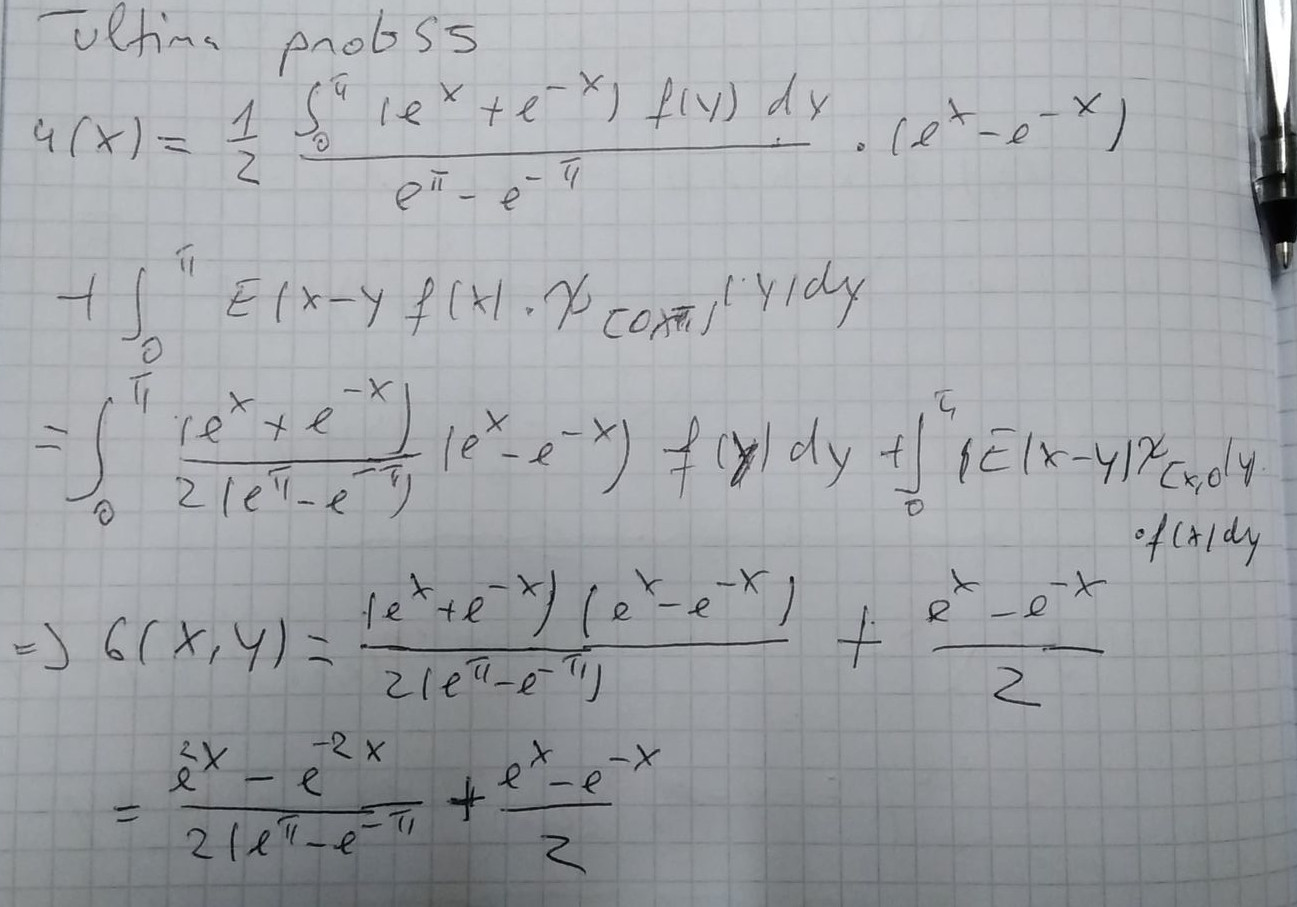
\includegraphics[width=\textwidth]{t.jpg}

      \medskip
      
      \textbf{Chestie folositoare:}

      cand aplici conditiile la limita, ai nevoie de formula:
      
      \[ \frac{d}{dx} \left (\int_{0}^{x} f(x,y)\,dy \right) = f\big(x,x) + \int_{0}^{x}\frac{\partial}{\partial x} f(x,y) \,dy\]

      \medskip
      
      care e obtinuta din formula Leibniz:
      \[ \frac{d}{dx} \left (\int_{a(x)}^{b(x)}f(x,t)\,dt \right) = f\big(x,b(x)\big)\cdot \frac{d}{dx} b(x) - f\big(x,a(x)\big)\cdot \frac{d}{dx} a(x) + \int_{a(x)}^{b(x)}\frac{\partial}{\partial x} f(x,t) \,dt\]

      
   

\end{document}
